\documentclass[UTF8,fontset=none,12pt]{ctexart}

\setCJKmainfont{Songti SC}
\setCJKsansfont{PingFang SC}
\setCJKmonofont{Songti SC}

\usepackage[a4paper,margin=2.35cm]{geometry}
\usepackage{amsmath,amssymb,amsthm,mathtools,bm}
\usepackage{graphicx}
\usepackage{float}
\usepackage{booktabs}
\usepackage{array}
\usepackage{enumitem}
\usepackage[hidelinks]{hyperref}

\title{数值线性代数\quad 第 36 讲：Lanczos 迭代}
\author{Lloyd N. Trefethen、David Bau III\quad 中文阅读版}
\date{}

\begin{document}
\maketitle
\pagestyle{plain}

前面三讲讨论了非 Hermitian 矩阵问题中的 Krylov 子空间迭代。第 39 讲还会
回到非 Hermitian 问题，因为这个主题远不止 Arnoldi 和 GMRES。不过在此之前，
本讲以及接下来的两讲专门讨论 Hermitian 情形；这时会出现一个巨大的简化。
为简化记号，本讲及后两讲进一步假设 $A$ 是实对称矩阵。

\section*{三项递推}

Lanczos 迭代就是专门用于 Hermitian 情形的 Arnoldi 迭代。前面第 33、34 讲
的所有公式仍然成立，只需把每个共轭转置 $^*$ 换成转置 $^T$。

首先，由式（33.12）可知 Ritz 矩阵 $H_n$ 是对称的。因此，它的特征值，也就是
Ritz 值或 Lanczos 估计（式（33.10）），都是实数。这很自然，因为 $A$ 的
特征值本来就是实数。

第二个观察更加重要：$H_n$ 既对称又是 Hessenberg 矩阵，所以它必然是三对角
矩阵。这意味着，在 Arnoldi 迭代（算法 33.1）的内层循环中，原本从 $1$ 到
$n$ 的求和范围可以缩短为从 $n-1$ 到 $n$。因此，在第 $n$ 步，不再需要
式（33.4）的 $(n+1)$ 项递推，而只需一个三项递推。结果是，每一步 Lanczos
迭代都比对应的 Arnoldi 步骤便宜得多。第 38 讲会看到类似现象：求解
$Ax=b$ 时，共轭梯度迭代的每一步也比 GMRES 的相应步骤便宜得多。

值得回顾的是，$H_n$ 为什么会变成三对角矩阵。对实矩阵 $A$、$H_n$ 和
$Q_n$，关键公式（33.12）可以按元素写成

\begin{equation}
h_{ij}=q_i^TAq_j.
\tag{36.1}
\end{equation}

由于 $Aq_j\in\operatorname{span}\{q_1,q_2,\ldots,q_{j+1}\}$，且 Krylov 向量
彼此正交，当 $i>j+1$ 时有 $h_{ij}=0$。取转置可得

\begin{equation}
h_{ij}=q_j^TA^Tq_i.
\tag{36.2}
\end{equation}

如果 $A=A^T$，用同样的推理可知当 $j>i+1$ 时 $h_{ij}=0$。由此得到三项
递推关系。这个论证不仅适用于矩阵，也适用于任意自伴算子。

\section*{Lanczos 迭代}

对称三对角矩阵只有两组不同的元素，因此通常不再使用一般的 $a_{ij}$ 记号。
令

\[
\alpha_n=h_{nn},\qquad
\beta_n=h_{n+1,n}=h_{n,n+1},
\]

于是 $H_n$ 记为

\begin{equation}
T_n=
\begin{bmatrix}
\alpha_1&\beta_1\\
\beta_1&\alpha_2&\beta_2\\
&\beta_2&\alpha_3&\ddots\\
&&\ddots&\ddots&\beta_{n-1}\\
&&&\beta_{n-1}&\alpha_n
\end{bmatrix}.
\tag{36.3}
\end{equation}

在这个记号下，算法 33.1 变成如下形式。

\begin{center}
\fbox{\begin{minipage}{0.88\textwidth}
\textbf{算法 36.1\quad Lanczos 迭代}

\[
\beta_0=0,\qquad q_0=0,\qquad
b\text{ 任意},\qquad q_1=b/\lVert b\rVert.
\]

\begin{enumerate}[leftmargin=2.6em,itemsep=0pt]
\item 对 $n=1,2,3,\ldots$：
\begin{enumerate}[label=\arabic*.,leftmargin=2.6em,itemsep=0pt]
\item $v=Aq_n$；
\item $\alpha_n=q_n^Tv$；
\item $v=v-\beta_{n-1}q_{n-1}-\alpha_nq_n$；
\item $\beta_n=\lVert v\rVert$；
\item $q_{n+1}=v/\beta_n$。
\end{enumerate}
\end{enumerate}
\end{minipage}}
\end{center}

为了提高稳定性，也可以在第 1 步先用
$v=Aq_n-\beta_{n-1}q_{n-1}$；此时第 3 步应改为只更新
$v\leftarrow v-\alpha_nq_n$，不能再次减去 $\beta_{n-1}q_{n-1}$。
这两种写法是等价的；这里把原书算法框中容易引起重复减法的括号说明展开写明。

每一步只包含一次矩阵--向量乘法、一次内积和少量向量运算。如果 $A$ 足够
稀疏，或者具有使矩阵--向量乘法便宜的其他结构，那么即使问题维数达到数万
乃至数十万，也可以相对容易地使用这种迭代。

下面的定理总结 Lanczos 迭代的若干性质。当然，和本书中所有这类定理一样，
它们是在精确算术下表述的。这里没有新的内容，只是把定理 33.1 和 34.1
改写为新的记号。

\textbf{定理 36.1.}
Lanczos 迭代生成的向量矩阵 $Q_n$ 是 Krylov 矩阵（式（33.6））的约化
QR 分解因子：

\begin{equation}
K_n=Q_nR_n.
\tag{36.4}
\end{equation}

三对角矩阵 $T_n$ 是对应的投影：

\begin{equation}
T_n=Q_n^TAQ_n.
\tag{36.5}
\end{equation}

连续迭代量满足

\begin{equation}
AQ_n=Q_{n+1}\widetilde T_n,
\tag{36.6}
\end{equation}

在第 $n$ 步，这可以写成三项递推

\begin{equation}
Aq_n=\beta_{n-1}q_{n-1}+\alpha_nq_n+\beta_nq_{n+1}.
\tag{36.7}
\end{equation}

只要 Lanczos 迭代没有发生 breakdown（即 $K_n$ 具有满列秩 $n$），$T_n$ 的
特征多项式就是唯一的 $p^n\in\mathcal P^n$，它解决 Arnoldi/Lanczos 逼近
问题（式（34.3）），即

\begin{equation}
\lVert p^n(A)b\rVert=\min.
\tag{36.8}
\end{equation}

\section*{Lanczos 与电荷分布}

在实践中，Lanczos 迭代和 Arnoldi 迭代用于非对称矩阵一样，常用于计算大型
对称矩阵的特征值（见第 34 讲）。在每一步 $n$，或者隔若干步，使用标准方法
计算不断增大的三对角矩阵 $T_n$ 的特征值。这些特征值就是给定矩阵 $A$ 和
初始向量 $q_1$ 的 Ritz 值或 Lanczos 估计（式（33.10））。通常可以观察到
其中一些数以几何速度收敛到某些极限；这些极限可以认为是 $A$ 的特征值。

和 Arnoldi 迭代一样，最先得到的通常是 $A$ 的离群特征值。这一说法可以用
下面的经验法则表达：

\begin{center}
\fbox{\begin{minipage}{0.86\textwidth}
如果 $A$ 的特征值比分布在区间上的 Chebyshev 点更加均匀，那么 Lanczos
迭代往往会首先找到离群特征值。
\end{minipage}}
\end{center}

为理解这句话，假设 $A$ 的 $m$ 个特征值 $\{\lambda_j\}$ 在实轴上的某个
区间内比较密集地分布。由于 Lanczos 迭代具有尺度不变性和平移不变性（定理
34.2），不妨假设区间是 $[-1,1]$。该区间内的 $m$ 个 Chebyshev 点定义为

\begin{equation}
x_j=\cos\theta_j,\qquad
\theta_j=\frac{(j-\tfrac12)\pi}{m},
\qquad 1\leq j\leq m.
\tag{36.9}
\end{equation}

这里精确的定义并不重要，重要的是：这些点在端点附近以二次方式聚集。点在
区间内部的间距为 $O(m^{-1})$，而在 $\pm1$ 附近的间距为 $O(m^{-2})$。
经验法则断言，如果 $A$ 的特征值比分布更均匀，即在端点附近聚集得更少，
那么 Lanczos 迭代计算出的 Ritz 值往往会首先收敛到离群特征值。特别地，
近似均匀的特征值分布会使离群值快速收敛。反过来，如果特征值比这更加
强烈地聚集在端点附近（实践中不太常见），则可能先收敛到某些“内部值”。

这些观察还可以作物理解释。考虑 $m$ 个可以在区间 $[-1,1]$ 内自由移动的
点电荷，假设位于 $x_j$ 和 $x_k$ 的电荷之间的排斥力与
$\lvert x_j-x_k\rvert^{-1}$ 成正比。（在三维空间中，电荷力通常与距离的
平方倒数成正比；但在二维中，可以把每个点看成三维中一条无限直线与平面
的交点，此时力与 $\lvert x_j-x_k\rvert^{-1}$ 成正比。）让这些电荷在
$[-1,1]$ 内达到最小能量平衡。这个最小能量分布与 Chebyshev 分布近似相同；
当 $m\to\infty$ 时，它们都趋于一个连续电荷密度

\[
\rho(x)\propto(1-x^2)^{-1/2}.
\]

把 $A$ 的特征值想象成点电荷。如果它们已经近似处于区间上的最小能量构型，
Lanczos 迭代就几乎没有用：在 $n=m$ 之前不会有多少收敛。反之，如果分布
与这种平衡状态差异很大，就可能快速收敛到某些特征值，即那些存在“电荷太少”
区域中的特征值。这里“电荷太少”的意思是：如果这些点可以自由移动，更多
电荷会倾向于聚集到该处。因此，经验法则也可以改写为：

\begin{center}
\fbox{\begin{minipage}{0.86\textwidth}
Lanczos 迭代倾向于收敛到平衡电荷分布中“电荷太少”的区域内的特征值。
\end{minipage}}
\end{center}

这一观察的解释依赖于式（36.8）所体现的 Lanczos 迭代与多项式逼近之间的
联系；习题 36.2 会展开其中一些细节。

\section*{例：离群特征值的快速收敛}

Lanczos 迭代的收敛可以用一个数值例子很好地说明。令 $A$ 为如下
$203\times203$ 矩阵：

\begin{equation}
A=\operatorname{diag}(0,.01,.02,\ldots,1.99,2,2.5,3.0).
\tag{36.10}
\end{equation}

$A$ 的谱由 $[0,2]$ 上的密集特征值以及两个离群值 $2.5$ 和 $3.0$ 组成。
从一个随机初始向量 $q_1$ 开始执行 Lanczos 迭代。

\begin{figure}[H]
\centering
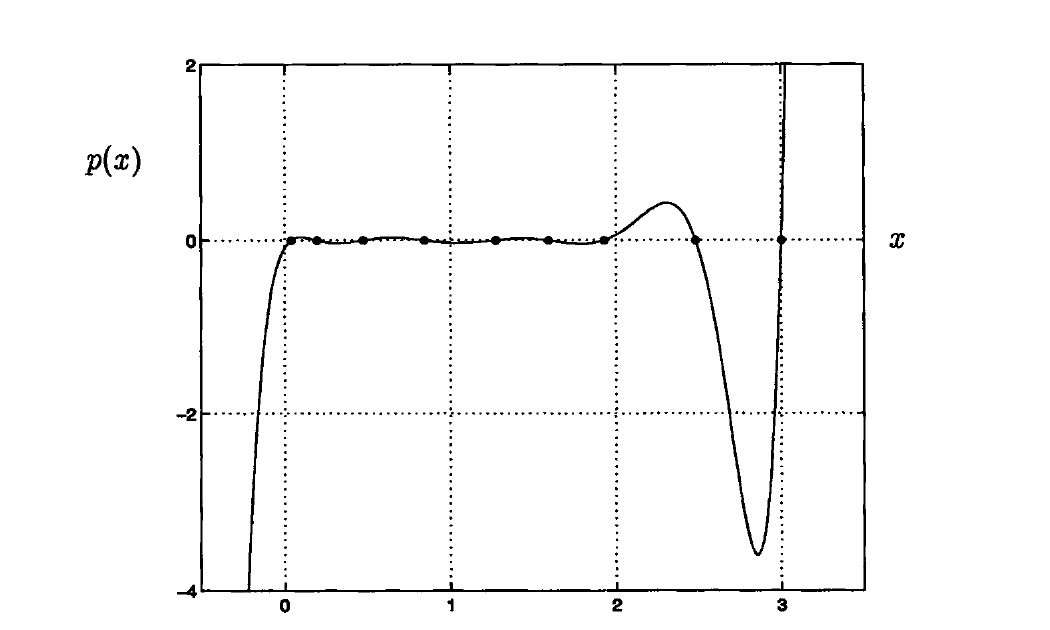
\includegraphics[width=0.82\textwidth]{../assets/figure-36-lanczos-polynomial.png}
\parbox{0.86\textwidth}{\small 图 36.1. 矩阵（36.10）的 Lanczos 迭代在第 9 步得到的 Lanczos 多项式。根是 Ritz 值，即 Lanczos 特征值估计。多项式在 $[0,2]\cup\{2.5\}\cup\{3.0\}$ 上都很小；因此它必须在 2.5 附近放置一个根，并在 3.0 附近放置另一个极近的根。}
\end{figure}

图 36.1 给出了第 $n=9$ 步的 Ritz 值及相应的 Lanczos 多项式。其中七个
Ritz 值位于 $[0,2]$ 内，多项式在该区间上几乎处处很小；还可以看出 Ritz
值开始向区间端点聚集。其余两个 Ritz 值分别靠近 $2.5$ 和 $3.0$。最大的
三个 Ritz 值为

\[
1.93,\qquad 2.48,\qquad 2.999962.
\]

可见，我们对较小特征值的精度还很低，但最大的特征值已经达到五位数字的
精度。这也说明了离群值为什么容易被准确估计：当 $x\approx3$ 时，$p(x)$
的图像非常陡。如果希望 $p(3)$ 很小，就必须有一个根非常接近 3。这种
陡峭性正对应于该点附近“电荷太少”的现象。如果这些电荷可以在 $[0,3]$
内自由移动以使能量最小，就会有更多点聚集在 $x=3$ 附近，而 $p(x)$ 在
那里就不会如此陡峭。

在第 20 步，最大的三个 Ritz 值为

\[
1.9906,\qquad
2.499999999987,\qquad
3.00000000000000.
\]

此时最大的特征值约有 15 位数字的精度，第二个约有 12 位。$p(x)$ 在
2.5 和 3.0 附近也会相应地变得陡峭。注意，第三个特征值也开始收敛；这反映
出 $[0,2]$ 内的特征值是均匀分布的，而不是 Chebyshev 分布。

图 36.2 给出了收敛过程的“俯视图”，显示 $n=1$ 到 $n=20$ 的所有 Ritz 值。
图中的每一条竖向切片对应一次迭代；连接散点的曲线只是帮助读者追踪变化，
没有严格的数学含义。图中显示，最大特征值在大约 $n=5$ 后出现明显收敛，
下一个特征值在 $n=10$ 左右开始收敛。在包含其余特征值的区间 $[0,2]$ 内，
Ritz 值的密度近似正比于 $(1-x^2)^{-1/2}$，并且在端点附近有明显聚集。

\begin{figure}[H]
\centering
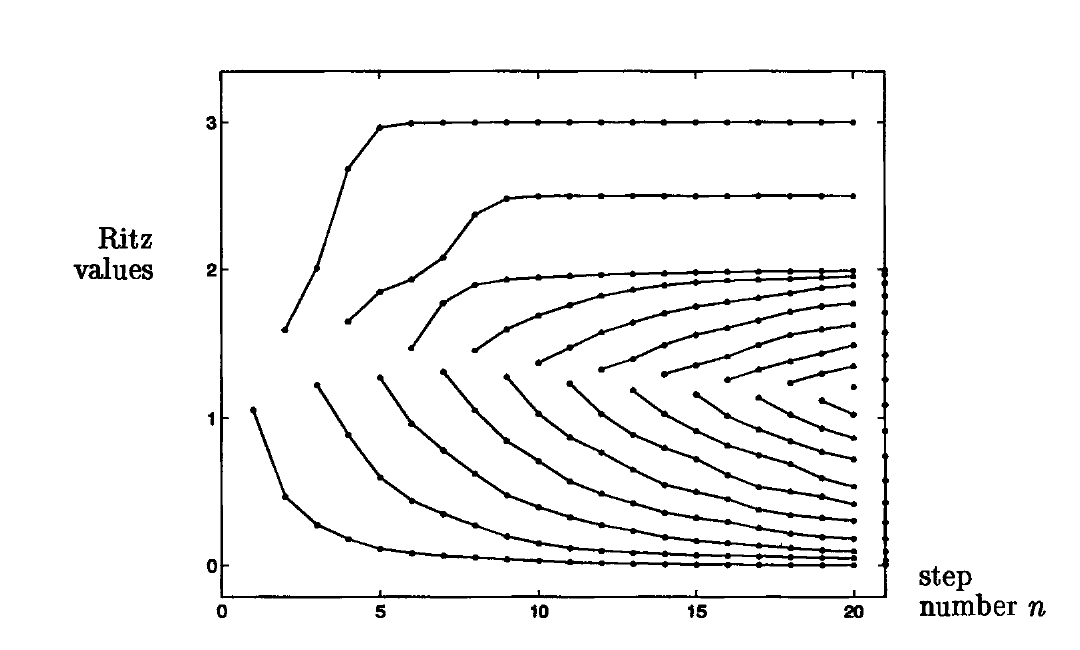
\includegraphics[width=0.90\textwidth]{../assets/figure-36-ritz-convergence.png}
\parbox{0.92\textwidth}{\small 图 36.2. 同一个矩阵上前 20 步 Lanczos 迭代的 Ritz 值。对特征值 2.5 和 3.0 的收敛是几何的；对 $[0,2]$ 中单个特征值的有效收敛很少，Ritz 值反而近似该区间上的 Chebyshev 点。}
\end{figure}

\section*{舍入误差与“幽灵”特征值}

舍入误差对 Lanczos 迭代以及所有基于三项递推的数值线性代数迭代都有复杂
影响。困难的来源很容易辨认：在 Arnoldi 或 GMRES 这样的 $n$ 项递推中，
向量 $q_1,q_2,q_3,\ldots$ 通过显式 Gram--Schmidt 运算被强制保持正交。
然而，Lanczos 和共轭梯度中的三项递推，依赖一个数学恒等式使向量
$\{q_i\}$ 的正交性“自动”出现。在实践中，舍入误差会使这些恒等式不能被
精确保持，经过若干步后，正交性就会丢失。

实践 Lanczos 迭代中正交性的丢失听起来完全是坏事，但实际情况更加微妙。
正交性丢失与 Ritz 值收敛到 $A$ 的特征值密切相关。关于这个主题已有大量
研究，但还没有给出本书意义下 Lanczos 或共轭梯度迭代稳定性的简单定理。
尽管如此，这些迭代在实践中仍然极其有用。图 36.3 展示了这种不稳定性通常
如何表现出来，而又不妨碍算法发挥作用。

\begin{figure}[H]
\centering
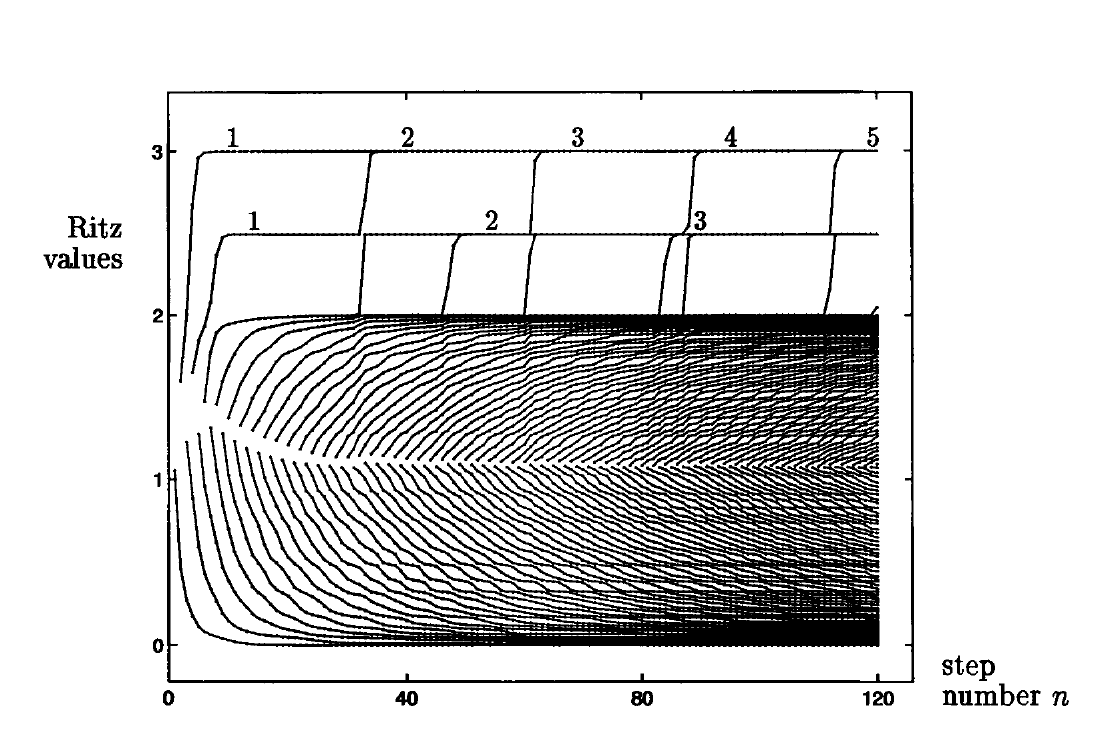
\includegraphics[width=0.90\textwidth]{../assets/figure-36-ghost-eigenvalues.png}
\parbox{0.92\textwidth}{\small 图 36.3. Lanczos 迭代延续到 120 步。图中数字表示 Ritz 值的重数；可以看到特征值 3.0 出现四个“幽灵”副本，特征值 2.5 出现两个“幽灵”副本。}
\end{figure}

图 36.3 是图 36.2 的重复版本，只是迭代从 20 步延长到了 120 步。在大约
第 30 步之前，一切都符合预期；随后，Ritz 值中出现了特征值 3.0 的第二个
副本。大约第 60 步出现第三个副本，第 90 步出现第四个副本，之后还会继续
出现。与此同时，特征值 2.5 的额外副本大约在第 40 步和第 80 步出现，并且
第 120 步也刚开始显现。这些额外的 Ritz 值称为“幽灵”特征值，与 $A$ 中
相应特征值的真实重数没有关系。

严格分析幽灵特征值现象很复杂，但直观解释并不难。一种解释是：在存在舍入
误差时，不应把 $A$ 的每个特征值看成一个点，而应看成一个长度大约为
$O(\varepsilon_{\mathrm{mach}}\lVert A\rVert)$ 的小区间。幽灵特征值出现，
是因为 $p(z)$ 不仅要在精确的特征值处很小，还要在这些小区间内处处很小。

另一种不同的解释是：Ritz 值收敛到 $A$ 的某个特征值时，会消灭当前运算向量
中对应的特征向量分量；但存在舍入误差时，随机噪声会再次轻微激发这个分量。
经过足够多次迭代后，这个此前被消灭的分量会被放大到足够大，于是需要另一个
Ritz 值再次把它消灭，然后还会再次、再次发生。

这两种解释都抓住了浮点算术中 Lanczos 迭代行为的部分真相；第二种解释也许
在定量上更准确。

\section*{习题}

\paragraph{36.1.}
第 27 讲指出，实对称矩阵 $A\in\mathbb R^{m\times m}$ 的特征值是 Rayleigh
商

\[
r(x)=\frac{x^TAx}{x^Tx},\qquad x\in\mathbb R^m
\]

的驻值。证明：如果把 $x$ 限制在 $\mathcal K_n$ 中，那么 Lanczos 迭代第
$n$ 步的 Ritz 值正好是 $r(x)$ 的驻值。

\paragraph{36.2.}
设 $p\in\mathcal P^n$，即

\[
p(z)=\prod_{k=1}^n(z-z_k),\qquad z_k\in\mathbb C.
\]

\begin{enumerate}[label=(\alph*)]
\item 将 $\log|p(z)|$ 写成对应于点 $z_k$ 的 $n$ 项之和。
\item 解释为什么包含 $z_k$ 的那一项可以看成位于 $z_k$ 的负单位点电荷所产生的势，其中电荷之间的排斥力与距离成反比。由此，$\log|p(z)|$ 可以看成 $n$ 个点电荷在 $z$ 处产生的势。
\item 将每个电荷 $-1$ 替换为 $-1/n$，并令 $n\to\infty$，得到总积分为 $-1$ 的连续电荷密度 $\mu(\zeta)$。写出表示其势 $\varphi(z)$ 的积分，并解释它与 $|p(z)|$ 的联系。
\item 设 $S$ 是 $\mathbb C$ 的闭有界子集且没有孤立点。假设我们寻找支撑在 $S$ 上、使 $\max_{z\in S}\varphi(z)$ 最小的分布 $\mu(z)$。给出一个非严格的论证，说明这样的 $\mu(z)$ 应满足 $\varphi(z)$ 在整个 $S$ 上为常数。解释这为何意味着“电荷”处于平衡状态、没有合力。换言之，$S$ 像一个二维导体，电荷总量 $-1$ 自由分布在其上；除一个加性常数外，$\varphi(z)$ 就是 $S$ 的 Green 函数。
\item 作为解释第 279 页经验法则的一步，设 $A$ 是实对称矩阵，其谱密集分布在
$[a,b]\cup\{c\}\cup[d,e]$，其中 $a<b<c<d<e$。于是对于集合 $S=[a,e]$，
$(b,d)$ 是“电荷太少”的区域。解释为什么可以期待 Ritz 值快速收敛到 $c$，
并用与集合 $S'=[a,b]\cup[c,d]$ 对应的平衡势 $\varphi(z)$ 估计收敛速率。
\end{enumerate}

\paragraph{36.3.}
设 $A$ 是 $1000\times1000$ 的对称矩阵，除下列元素外均为 0：对角元
$a_{ii}=\sqrt{i}$；次对角线和超对角线上的元素为 1；第 100 条次对角线和
超对角线上的元素也为 1，即当 $|i-j|=100$ 时 $a_{ij}=1$。用 Lanczos
迭代将 $A$ 的最小特征值计算到六位有效数字。

\paragraph{36.4.}
作为第 34 讲 Arnoldi 纽结线的特例，可以使用“Lanczos 纽结线”来说明
Lanczos 迭代的收敛。想办法修改习题 36.3 的程序，使它能够在每一步绘制
Lanczos 纽结线。方法不必优雅、高效或数值稳定。对图 36.2 的例子以及一个
自行选择的例子，分别绘制 $n=1,2,\ldots,12$ 步的 Lanczos 纽结线。

\end{document}
